\documentclass[12pt,letterpaper]{article}

\usepackage[table]{xcolor}
\usepackage[margin=1in]{geometry}
\usepackage{fancyhdr}
\usepackage{amsmath}
\usepackage{tikz}
\usepackage{tabularx}
\usepackage{changepage}
\DeclareUnicodeCharacter{2217}{*}
\pagestyle{fancy}
\rhead{Homework 2}
\lhead{\textbf{Phien Nguyen}}

\begin{document}
\section{Dijkstra’s algorithm}
Consider the following graph. Let the start vertex be xs and the goal vertex be xg. Important: if a
node has multiple outgoing edges, when the node is expanded the vertices adjacent to the node are
processed in alphabetical order. Similarly, if multiple nodes in the OPEN queue have the same
priority value, sort them by alphabetical order.
\\
\\
\begin{tabularx}{1\textwidth} {
        | >{\centering\arraybackslash}X
        | >{\centering\arraybackslash}X
        | >{\centering\arraybackslash}X
        | >{\centering\arraybackslash}X
        | >{\centering\arraybackslash}X
        | >{\centering\arraybackslash}X
        | >{\centering\arraybackslash}X
        | >{\centering\arraybackslash}X
        | >{\centering\arraybackslash}X
        | >{\centering\arraybackslash}X
        | >{\centering\arraybackslash}X | }
    \hline
        Step & $x_{s}$ & A & B & C & D & E & F & G & H & $x_{g}$
        \\
    \hline
        0 & N/0 & $\infty$ & $\infty$ & $\infty$ & $\infty$ & $\infty$ & $\infty$ & $\infty$ & $\infty$ & $\infty$
        \\
    \hline
        1 & N/0 & $x_{s}$/1 & $x_{s}$/5 & $x_{s}$/3 & $\infty$ & $\infty$ & $\infty$ & $\infty$ & $\infty$ & $\infty$
        \\
    \hline
        2 & N/0 & $x_{s}$/1 & A/2 & $x_{s}$/3 & A/5 & B/9 & C/4 & $\infty$ & $\infty$ & $\infty$
        \\
    \hline
        3 & N/0 & $x_{s}$/1 & A/2 & $x_{s}$/3 & B/4 & B/6 & C/4 & $\infty$ & $\infty$ & $\infty$
        \\
    \hline
        4 & N/0 & $x_{s}$/1 & A/2 & $x_{s}$/3 & B/4 & D/5 & C/4 & D/6 & F/7 & $\infty$
        \\
    \hline
        5 & N/0 & $x_{s}$/1 & A/2 & $x_{s}$/3 & B/4 & D/5 & C/4 & D/6 & F/7 & F/5
        \\
    \hline
\end{tabularx}


\begin{figure}[!h]
\centering
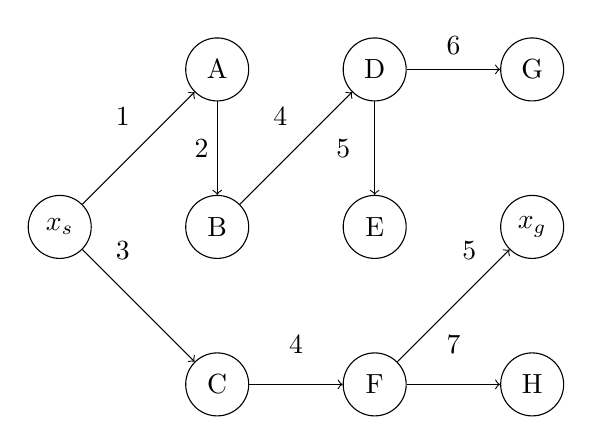
\begin{tikzpicture}[
        main node/.style={circle, draw, minimum size=.8cm,inner sep=0pt},
    ]

    \node[main node] (xs) at (0,2) {$x_{s}$};
    \node[main node] (A) at (2,4) {A};
    \node[main node] (B) at (2,2) {B};
    \node[main node] (C) at (2,0) {C};
    \node[main node] (D) at (4,4) {D};
    \node[main node] (E) at (4,2) {E};
    \node[main node] (F) at (4,0) {F};
    \node[main node] (G) at (6,4) {G};
    \node[main node] (H) at (6,0) {H};
    \node[main node] (xg) at (6,2) {$x_{g}$};

    \node(xs2A) at (.8, 3.4)    {1};
    \node(A2B) at (1.8, 3)      {2};
    \node(xs2C) at (.8, 1.7)    {3};
    \node(xs2C) at (3, .5)      {4};
    \node(F2G) at (5, .5)       {7};
    \node(F2xg) at (5.2, 1.7)   {5};
    \node(B2D) at (2.8, 3.4)    {4};
    \node(D2E) at (3.6, 3)      {5};
    \node(D2G) at (5, 4.3)      {6};

    \draw[->] (xs) -- (A);
    \draw[->] (xs) -- (C);
    \draw[->] (A) -- (B);
    \draw[->] (C) -- (F);
    \draw[->] (F) -- (H);
    \draw[->] (F) -- (xg);
    \draw[->] (B) -- (D);
    \draw[->] (D) -- (E);
    \draw[->] (D) -- (G);
\end{tikzpicture}
\end{figure}

\section{A$^{\ast}$}
Consider the directed weighted graph shown at page 2.
Show how the algorithm A∗ would determine the shortest path between xs and xg. Follow the
same method used in class and in example 4.5 in the lecture notes.
\\
\\
\begin{adjustwidth}{-1.2cm}{}
    \begin{tabularx}{1.15\textwidth} {
            | >{\centering\arraybackslash}X
            | >{\centering\arraybackslash}X
            | >{\centering\arraybackslash}X
            | >{\centering\arraybackslash}X
            | >{\centering\arraybackslash}X
            | >{\centering\arraybackslash}X
            | >{\centering\arraybackslash}X
            | >{\centering\arraybackslash}X
            | >{\centering\arraybackslash}X
            | >{\centering\arraybackslash}X | }
        \hline
            OPEN & $x_{s}$ & A & B & C & D & E & F & G & $x_{g}$
            \\
        \hline
            $x_{s}$ & N/0/7 & $N/\infty/\infty$ & $N/\infty/\infty$ & $N/\infty/\infty$ & $N/\infty/\infty$ & $N/\infty/\infty$ & $N/\infty/\infty$ & $N/\infty/\infty$ & $N/\infty/\infty$
            \\
        \hline
            F,A,B & $x_{s}$ & $x_{s}/2/14$ & $x_{s}/3/14$ & $N/\infty/\infty$ & $N/\infty/\infty$ & $N/\infty/\infty$ & $x_{s}/5/11$ & $N/\infty/\infty$ & $N/\infty/\infty$
            \\
        \hline
            F,A,B & $x_{s}$ & $x_{s}/2/14$ & $x_{s}/3/14$ & $N/\infty/\infty$ & $N/\infty/\infty$ & $N/\infty/\infty$ & $x_{s}/5/11$ & $N/\infty/\infty$ & $N/\infty/\infty$
            \\
        \hline
            F & $x_{s}$ & $x_{s}/2/14$ & $x_{s}/3/14$ & $F/7/14$ & $N/\infty/\infty$ & $F/9/13$ & $x_{s}/5/11$ & $N/\infty/\infty$ & $N/\infty/\infty$
            \\
        \hline
            E, C & $x_{s}$ & $x_{s}/2/14$ & $x_{s}/3/14$ & $F/7/14$ & $E/10/14$ & $F/9/13$ & $x_{s}/5/11$ & $E/16/14$ & $C/17/14$
            \\
        \hline
            D & $x_{s}$ & $x_{s}/2/14$ & $x_{s}/3/14$ & $F/7/14$ & $E/10/14$ & $F/9/13$ & $x_{s}/5/11$ & $E/16/14$ & $D/12/14$
            \\
        \hline
    \end{tabularx}
\end{adjustwidth}

\section{Navigation functions 1}

$$
    \begin{tabularx}{.4\textwidth} {
            | >{\centering\arraybackslash}X
            | >{\centering\arraybackslash}X
            | >{\centering\arraybackslash}X
            | >{\centering\arraybackslash}X
            | >{\centering\arraybackslash}X
            | >{\centering\arraybackslash}X
            | >{\centering\arraybackslash}X
            | >{\centering\arraybackslash}X
            | >{\centering\arraybackslash}X
            | >{\centering\arraybackslash}X | }
        \hline
            8 & 7 & 6 & 5 & 4 & 3 & 2 & 1 & 2 & 3
            \\
        \hline
            7 & 6 & 5 & 4 & 3 & 2 & 1 & 0 & 1 & 2
            \\
        \hline
            8 & 7 & 6 & 5 & 4 & 3 & 2 & 1 & 2 & 3
            \\
        \hline
            \cellcolor{black} & \cellcolor{black} & 7 & 6 & 5 & \cellcolor{black} & \cellcolor{black} & 2 & 3 & 4
            \\
        \hline
            10 & 9 & 8 & 7 & 6 & 5 & 4 & 3 & 4 & 5
            \\
        \hline
            11 & 10 & 9 & 8 & \cellcolor{black} & \cellcolor{black} & 5 & 4 & 5 & 6
            \\
        \hline
            12 & \cellcolor{black} & \cellcolor{black} & \cellcolor{black} & \cellcolor{black} & \cellcolor{black} & 6 & 5 & 6 & 7
            \\
        \hline
            13 & \cellcolor{black} & \cellcolor{black} & \cellcolor{black} & \cellcolor{black} & \cellcolor{black} & 7 & 6 & 7 & 8
            \\
        \hline
            14 & 13 & 12 & 11 & 10 & 9 & 8 & \cellcolor{black} & \cellcolor{black} & 9
            \\
        \hline
            15 & 14 & 13 & 12 & 11 & 10 & 9 & 10 & 11 & 10
            \\
        \hline
    \end{tabularx}
$$

\section{Navigation functions 2}

1. Visually, the greatest offender of the navigation function is that bottom left the numbers jump from 10 to 15. There are other instances where the numbers are not adding up properly like on the left side again with the 10 and 7. There are also the bottom right as 6 goes to 9 then 8 which is wrong.
\\
\\
2.
$$
    \begin{tabularx}{.4\textwidth} {
            | >{\centering\arraybackslash}X
            | >{\centering\arraybackslash}X
            | >{\centering\arraybackslash}X
            | >{\centering\arraybackslash}X
            | >{\centering\arraybackslash}X
            | >{\centering\arraybackslash}X
            | >{\centering\arraybackslash}X
            | >{\centering\arraybackslash}X | }
        \hline
            6 & 5 & 4 & 3 & 2 & 1 & 2 & 3
            \\
        \hline
            7 & 6 & \cellcolor{black} & 2 & 1 & 0 & \cellcolor{black} & \cellcolor{black}
            \\
        \hline
            8 & 7 & \cellcolor{black} & 3 & 2 & 1 & 2 & 3
            \\
        \hline
            9 & 8 & \cellcolor{black} & \cellcolor{black} & 3 & 2 & 3 & 3
            \\
        \hline
            10 & \cellcolor{green}9 & \cellcolor{black} & 5 & 4 & 3 & 4 & 5
            \\
        \hline
            9 & \cellcolor{green}10 & \cellcolor{black} & 6 & 5 & 4 & 5 & 6
            \\
        \hline
            10 & 9 & 8 & 7 & 6 & 5 & \cellcolor{black} & 7
            \\
        \hline
            \cellcolor{green}11 & 10 & 9 & 8 & 7 & 6 & \cellcolor{green}7 & 8
            \\
        \hline
    \end{tabularx}
$$

\end{document}
